\documentclass[utf8x, 12pt]{G7-32} 


% --------- -------- SETTINGS --------- --------

% --------- Настройки стиля ГОСТ 7-32 --------

% Гипертекстовое оглавление в PDF
\usepackage[
bookmarks=true, colorlinks=true, unicode=true,
urlcolor=black,linkcolor=black, anchorcolor=black,
citecolor=black, menucolor=black, filecolor=black,
]{hyperref}

\usepackage{graphicx}   % Пакет для включения рисунков
\DeclareGraphicsExtensions{.jpg,.pdf,.png}
\geometry{right=20mm}
\geometry{left=30mm}
\usepackage{enumerate}
\setcounter{tocdepth}{3} % Подробность оглавления


% --------- other settings --------
\usepackage{MnSymbol}
%\usepackage{simpsons}
% --------- -------- SETTINGS --------- --------

% LISTINGS
\usepackage{listings}
\usepackage{color}

\definecolor{dkgreen}{rgb}{0,0.6,0}
\definecolor{gray}{rgb}{0.5,0.5,0.5}
\definecolor{mauve}{rgb}{0.58,0,0.82}

\lstset{frame=tb,
  language=bash,
  aboveskip=3mm,
  belowskip=3mm,
  showstringspaces=false,
  columns=flexible,
  basicstyle={\small\ttfamily},
  numbers=none,
  numberstyle=\tiny\color{gray},
  keywordstyle=\color{blue},
  commentstyle=\color{dkgreen},
  stringstyle=\color{mauve},
  breaklines=true,
  breakatwhitespace=true,
  tabsize=3
}

\begin{document}

\frontmatter 

% --------- -------- TITLE --------- --------

\begin{center} 

\large САНКТ-ПЕТЕРБУРГСИЙ ГОСУДАРСТВЕННЫЙ ПОЛИТЕХНИЧЕСКИЙ УНИВЕРСИТЕТ

\large Кафедра Компьютерных Систем и Программных Технологий \\[5.5cm] 

\huge ОТЧЕТ \\[0.6cm] % название работы, затем отступ 0,6см
\large по лабораторной работе №8\\
\large Тема: <<Проект OWASP WebGoat>>\\
\large Дисциплина: <<Методы и средства защиты информации>>\\[3.7cm]

\end{center} 

\begin{flushright}
Выполнил: студент гр. 53501/2 \\
Федоров Е.М. \\[1.2cm]


Преподаватель \\
Вылегжанина К.Д.
\end{flushright}


\vfill 

\begin{center} 
\large Санкт-Петербург \\
2015
\end{center} 

\thispagestyle{empty}


% --------- -------- TITLE --------- --------

\thispagestyle{empty}
\setcounter{page}{0}
\tableofcontents
\clearpage
\mainmatter


\chapter{Задание}
Запустить уязвимое приложение WebGoat. Запустить сканер безопасности ZAP. Запустить инструмент Mantra, настроить его для использования ZAP в качестве прокси--сервера. Изучить:

\begin{enumerate}
	\item Недостатки контроля доступа
	\item Безопасность AJAX
	\item Недостатки аутентификации
	\item Переполнение буфера
	\item Качество кода
	\item Многопоточность
	\item Межсайтовое выполнение сценариев
	\item Неправильная обработка ошибок
	\item Недостатки приводящие к осуществлению инъекций (SQL и прочее)
	\item Отказ в обслуживании
	\item Небезопасное сетевое взаимодействие
	\item Небезопасная конфигурация
	\item Небезопасное хранилище
	\item Исполнение злонамеренного кода
	\item Подделка параметров
	\item Недостатки управление сессией
	\item Безопасность веб--сервисов
\end{enumerate}

\chapter{Выполнение работы}

\section{Изучение}
\subsection{Описания десяти самых распространенных веб-уязвимости согласно рейтингу OWASP}

\begin{itemize}
\item {\textbf{Injection} Атака на интепритатор машины-цели, позволяя выполнять произвольный код от ее имени. Чаще всего встрачаются в SQL, LDAP, Xpath, или NoSQL запросах, парсерах xml, аргументах программ и т.д.}

\item {\textbf{Broken Authentication and Session Management} Атака на уязвимости систем авторизации и управления сессиями с целью кражи и/или выполнения каких либо действий от чужого имени.}

\item {\textbf{Cross-Site Scripting} Атака на браузер путем подмены загружаемых скриптов. В результате злоумышлиниками может быть получена почти любая информация.}

\item {\textbf{Insecure Direct Object References} Суть атаки - изменение некого объекта, используемого в авторизированной сессии. 

Изменение параметра позволит отправлять измененные запросы от имени авторизированного пользователя.}

\item {\textbf{Security Misconfiguration} Ошибки в конфигурации. Атакующий может получить доступ к файлам, акаунтам, системе и т.д.}

\item {\textbf{Sensitive Data Exposure} Кража ценной/личной информации. Атака сложна если используется шифрование. В таком случае данные крадутся косвенными методами: на стороне клиента, когда данные уже рашифрованы, man-in-the-middle атака и другими способами.}

\item {\textbf{Missing Function Level Access Control} Доступ неавторизированного пользователя к привелегированным функциям. 
Пример: 

\begin{lstlisting}
\begin{Verbatim}[frame=single]
http://example.com/app/getappInfo
http://example.com/app/admin_getappInfo <<<<
\end{lstlisting}
Доступ к функции admin\_getappInfo должен иметь только администратор. Соответственно, если пользователь, не являющийся администритором получает доступ к данной функции - это уязвимость.}

\item {\textbf{Cross-Site Request Forgery} Атака путем выполнения запросов к некоторому защищенному ресурсу от его имени авторизованного пользователя. Недостаток - атакующий не может перехватить ответ от ресурса. В этом случае вводят так называемые CSRF-токены: каждый последующий пакет от клиента содержит токен, полученный в пердыдущем ответе сервера.}

\item {\textbf{Using Components with Known Vulnerabilities} Атака на уязвимый компонент системы, выявленный в результате сканирования.}

\item {\textbf{Unvalidated Redirects and Forwards} Скрытые ссылки в картинках, фреймах и т.д., ведущих на доверенный сайт. Позволяет произвести любой запрос.
Пример:
\begin{lstlisting}
http://www.example.com/redirect.jsp?url=evil.com
\end{lstlisting}
}
\end{itemize}

\newpage
\section{Запуск WebGoat, ZAP, Mantra}

\begin{figure}[hhh!]
\centering
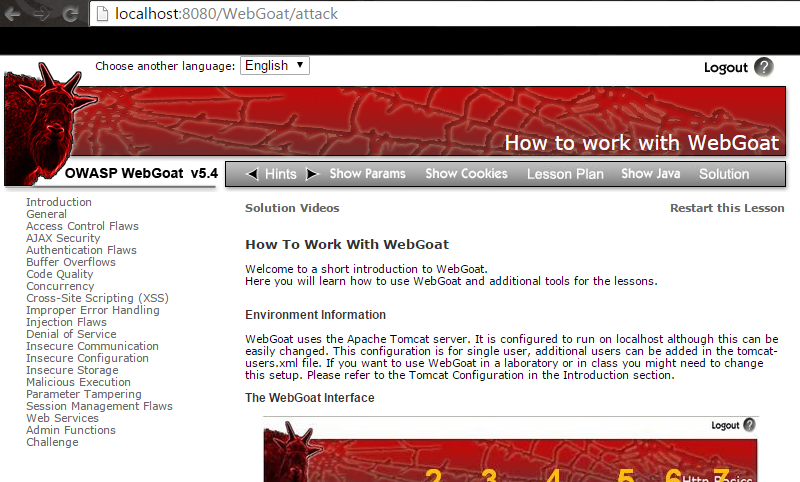
\includegraphics[width=12cm]{rsrc/webgoat_start}
\caption{WebGoat запущен на порту 8080. Системные настройки http прокси-сервера установлены в localhost:8081}
\end{figure}

\begin{figure}[hhh!]
\centering
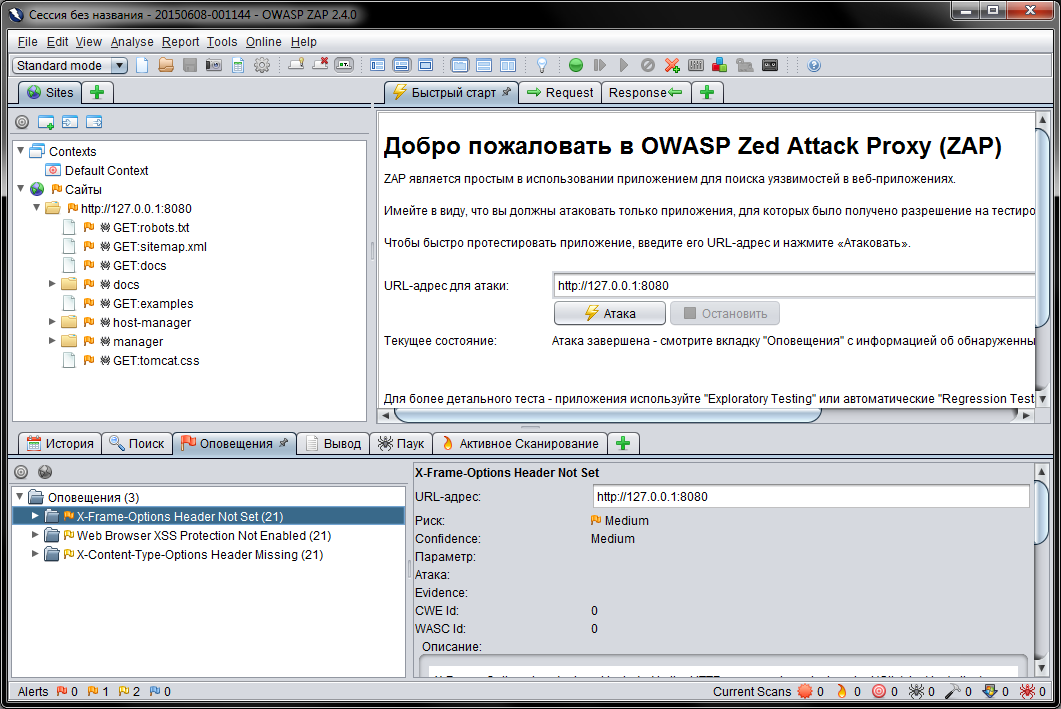
\includegraphics[width=12cm]{rsrc/zap_start}
\caption{ZAP запущен. Поднят локальный прокси-сервер на порту 8081.}
\end{figure}

\begin{figure}[hhh!]
\centering
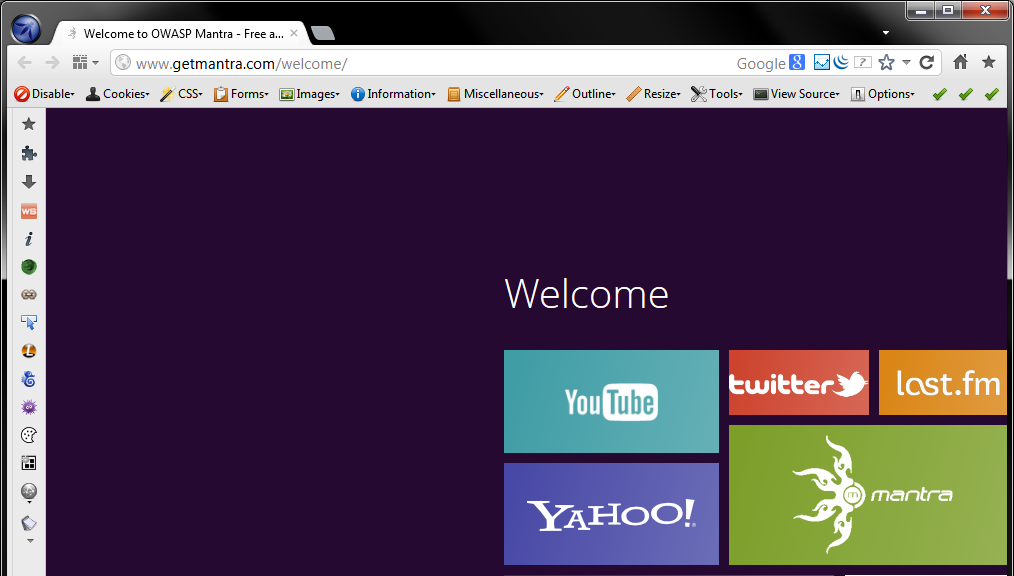
\includegraphics[width=12cm]{rsrc/mantra_start}
\caption{Mantra запущен. Переход на любой сайт отображается в ZAP в виде перехваченных данных. Все работает нормально.}
\end{figure}

\newpage
\section{Basics}

Сначала переводим ZAP в режим прослушивания и перехвата, нажав плюсик рядом со вкладкой Response, а затем нажав кнопку Set break on all requests.


\begin{figure}[hhh!]
\centering
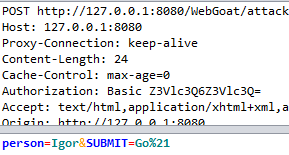
\includegraphics[width=10cm]{rsrc/1_2}
\caption{В ZAP видим перехваченные данные. Чтобы имя не было перевернуто, изменим его в ZAP на rogI и отправим. Урок пройден.}
\end{figure}


\newpage
\section{Недостатки контроля доступа}
\begin{figure}[hhh!]
\centering
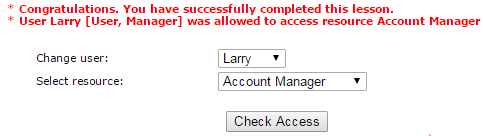
\includegraphics[width=12cm]{rsrc/2_1}
\caption{Находим пользователя Larry, у которого есть доступ к ресурсу Account Manager, хотя его быть не должно.}
\end{figure}


Во второй части этого урока мы получаем доступ к файлу, находящемуся вне нашей директории. Для этого перехватим запрос как это было сделано ранее. В списке выберем любой файл и нажмем View File. В окне ZAP заменим имя файла на строку "/../../../../conf/tomcat-users.xml". Доступ к файлу получен.

В третьей части урока заходим под аккаунтом админа John:john и выясняем, что метод для удаления пользователей называется DeleteProfile. Затем заходим под аккаунтом Tom:tom и перехватывая запрос View Profile подменим вызываемый метод на DeleteProfile. Профиль другого сотрудника удален. 
Второй и четвертый шаги не выполнить, поскольку версия WebGoat не Developers. На третьем шаге авторизируемся под аккаунтом Tom:tom и выбирая в списке себя, нажимаем кнопку View Profile. Перехватывая этот запрос в ZAP подменим аргумент employee\_id на другой, например, 107. Информация о другом сотруднике получена.

В четвертой части урока нам надо попытаться получить информацию, доступную только админу. Заходя на вкладки User Information и Product Information мы добавляем в адресную строку к нашему запросу еще один аргумент: admin=true.


\begin{figure}[hhh!]
\centering
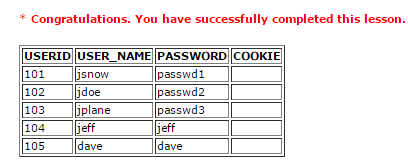
\includegraphics[width=7cm]{rsrc/3_1}
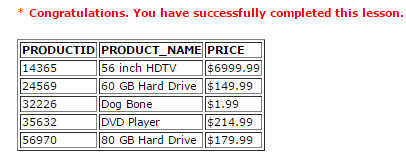
\includegraphics[width=7cm]{rsrc/3_2}
\caption{Доступ к User Information получен.}
\end{figure}

\newpage
\section{Безопасность AJAX}
Первая часть урока объясняет почему запросы могут отсылаться только серверу-отправителю страницы. Это сделано для повышения безопасности, но может быть отключено. Современные браузеры блокируют загрузку сторонних скриптов. 

Вторая часть урока наглядно показывает, что необходимо экранировать поля ввода. В данном случае можно легко подменить текст произвольным html кодом.
\begin{figure}[hhh!]
\centering
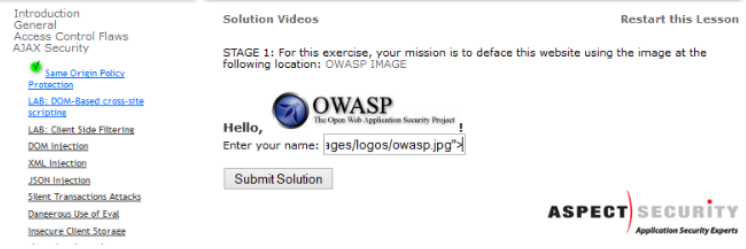
\includegraphics[width=\textwidth]{rsrc/4_1}
\caption{Заменили имя на ссылку на картинку.}
\end{figure}

Третья часть урока показывает, что необходимо делать валидацию данных не только на клиенте, но и на сервере, чтобы исключить подмену ajax-запросов. Изменив скрипт обработки запроса мы исключили возможность выдачи лишних данных клиенту.

Четвертая часть урока поясняет принцип работы DOM injection. Используя инъекцию меняем свойство кнопки submit.disabled на false при помощи перехвата запроса и инъекции следующей строки:
\begin{lstlisting}
document.forms[0].SUBMIT.disabled=false;
\end{lstlisting}
Кнопка становится активной.\\

Пятая часть урока затрагивает XML injection. Нам предлагается выбрать себе награду, введя свой ID. Запускаем ZAP, перехватывает запрос, вводя свой номер. Правим XML-код, добавляя себе награды используя тег <reward></reward>.
\begin{figure}[h!]
\centering
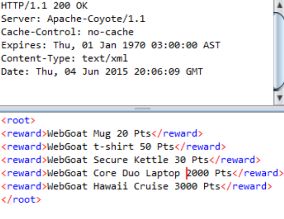
\includegraphics[width=0.4\textwidth]{rsrc/5_1}
\caption{Добавляем себе наград.}
\end{figure}

\newpage
Шестая часть урока про JSON injection. Аналогично предыдущим вариантам подменяем JSON код, перехватывая запрос. Выбираем лучшую цену.

Седьмая часть - не стоит делать проверку на клиентской стороне. Необходимо найти клиентскую функцию для отправки и вызвать ее.
\begin{lstlisting}
submitData(555, 1000000)
\end{lstlisting}

Восьмая часть аналогична: убираем readonly и отмечаем GOLD, стоимость покупок = 0.

В девятой части описывается опасность использования функции eval. Вводим в поле код
\begin{lstlisting}
`)%3Balert(document.cookie%2B'something
\end{lstlisting}


\newpage
\section{Недостатки аутентификации}

Абсолютно очевидно, что сложность подбора пароля зависит от его длины и набора символов.
Вторая часть урока показывает, что слишком простые способы восстановления делают любой пароль уязвимым. Можно с легкостью подобрать ответ на секретный вопрос типа ''Ваш любимый цвет''.

Часть Basic Authentication показывает как можно легко расшифровать содежимое заголовка, раскодировав содержимое его значения из base64 в простой текст. Получили guest:guest. В настройках браузера чистим куки и данные сессий и логинимся как basic:basic.

В третьей части плохо реализованная многоуровневая защита. Перехватываем данные, изменяем hiddentan=1. Обошли защиту.

В четвертой части опять многоуровневая защита, авторизация под аккаунтом Joe, ввводим его tan, Перехватываем данные, в запросе указываем Jane.

\section{Переполнение буфера}
Перехватываем пакет с помощью ZAP, добавляем в значение аргумента roomno >4096 символов.
\begin{figure}[h!]
\centering
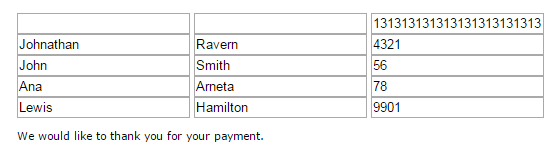
\includegraphics[width=\textwidth]{rsrc/6_1}
\caption{Запоминаем какого-либо пользователя, заходим от его имени.}
\end{figure}


\section{Качество кода}
В коде страницы можно найти логин и пароль администратора: admin:adminpw.

\section{Многопоточность}
В первой части при одновременном получении данных пользователя возможна их утечка. Можн ополучить чужие данные. Открываем два окна и вводим имена пользователей. В некоторых ситуациях можно получить не свою информацию.

Во второй части открываем два окна, в одном делаем большую покупку, в другом- маленькую, Продолжаем маленькую покупку и обновляем большую. При подтверждении платим за маленькую, а получаем большую покупку.


\section{Межсайтовое выполнение сценариев}
С помощью XSS и HTML можно заменять элементы страницы на фиктивные, а пользователь даже не поймет что что-то изменилось.
\begin{figure}[h!]
\centering
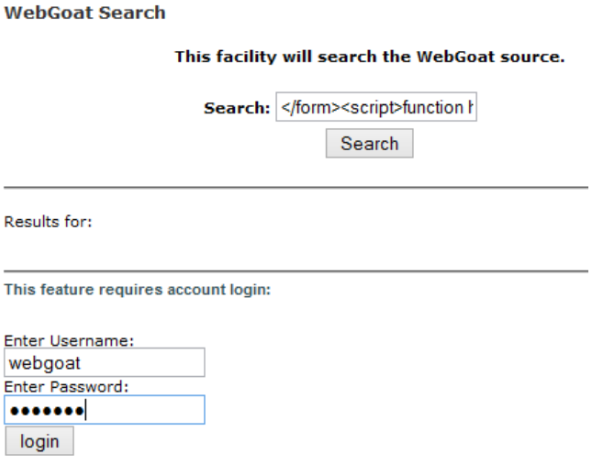
\includegraphics[width=12cm]{rsrc/7_1}
\caption{Использование XSS.}
\end{figure}

\section{Неправильная обработка ошибок}
В перехваченном пакете достаточно удалить поле пароля и авторизация пройдет успешно.


\section{Недостатки приводящие к осуществлению инъекций}
\begin{itemize}
\item Command injection
Перехватываем запрос, добавляем к имени файла строку:
\begin{lstlisting}
%22%3B%20netstat%20-a
\end{lstlisting}
\item Numeric SQL injection
Перехватываем запрос. Модифицируем:
\begin{lstlisting}
station=101or%201%3D1&SUBMIT=Go!
\end{lstlisting}
\item Log spoofing
Перехватываем запрос, меняем имя на следующее:
\begin{lstlisting}
somename
Admin succefully entered!
\end{lstlisting}
В результате, в логе создается видимость того, что админ авторизовался.
\item SQL Injection
Перехватываем сообщение. В качестве пароля вводим:
\begin{lstlisting}
123123%27%20OR%20%271%27%3D%271
\end{lstlisting}
При попытке получить данные на втором шаге получаем сообщение:
\begin{lstlisting}
THIS LESSON ONLY WORKS WITH THE DEVELOPER VERSION OF WEBGOAT
\end{lstlisting}
\item String sql injection
Аналогично. Вместо имени вводим 123123' OR 'a' = 'a. Получаем все возможные значения.
\item Modify Data with SQL INJECTION
Вместо имени вводим:
\begin{lstlisting}
123'; UPDATE salaries SET salary=5 
WHERE userid='jsmith
\end{lstlisting}
\item Database backdoors
По такой же схеме можно добавлять и триггеры:
\begin{lstlisting}
101; CREATE TRIGGER myBackDoor BEFORE INSERT ON
 employee FOR EACH ROW BEGIN UPDATE employee 
 SET email='john@hackme.com' WHERE userid = NEW.userid
\end{lstlisting}
\end{itemize}

\section{Отказ в обслуживании}
В пункте ZipBomb создается файл zip, содержащий большое количество одинаковых символов. При распаковке потребление памяти станет огромным из-за большой степени сжатия.

В пункте DoS from Multiple logins вместо пароля вводим
\begin{lstlisting}
pewpew' or `1' or `1
\end{lstlisting}
Получаем
\begin{lstlisting}
101 jsnow passwd1
102 jdoe passwd2
103 jplane passwd3
104 jeff jeff
105 dave dave
\end{lstlisting}
Авторизуемся этими данными. Получаем отказ в обслуживании из-за большого количества сессий.

\section{Небезопасное сетевое взаимодействие}
При передаче пароля вне защищенного соединения его можно легко перехватить, для избежания этого необходимо использовать https + TLS. Пароль можно получить перехватив запрос аутентификации.

\section{Небезопасная конфигурация}
У большинства сайтов есть панель администрирования. Если она будет расположена в очевидном месте, можно легко получить к ней доступ, следовательно неоходимо скрыть ее местонахождение. В данном случае она находится в директории WebGoat/conf.


\section{Небезопасное хранилище}
Различные кодировки строк, лучше хранить данные в зашифрованном виде. Тогда даже при утечке с ними сложно что-либо сделать.
\begin{figure}[h!]
\centering
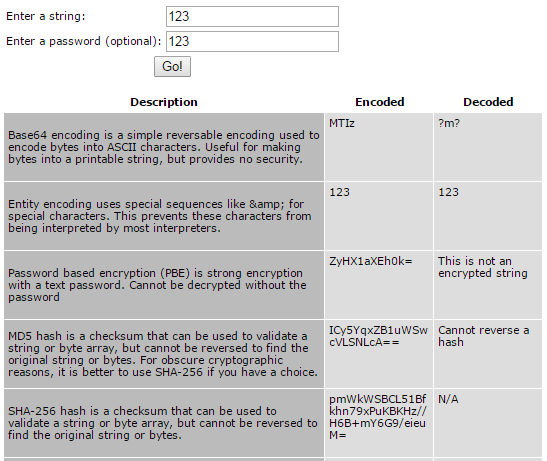
\includegraphics[width=\textwidth]{rsrc/8_1}
\caption{Строка ''123'' в различных кодировках.}
\end{figure}


\section{Исполнение злонамеренного кода}
Если злоумышленнику известна директория с исполняемыми файлами, то он может загрузить туда свой код и исполнить его.
Загрузим на сервер скрипт со следущим содержанием
\begin{lstlisting}
<html>
<%
java.io.File fil = new java.io.File(''D:\WebGoat-5.4\tomcat
\webapps\WebGoat\mfe_target\guest.txt'');
file.createNewFile();
%>
</html>
\end{lstlisting}

\newpage
\section{Подделка параметров}
В части Bypass HTML Field Restrictions необходимо в перехваченном сообщении поменять значение всех полей и добавить  disabledinput.

Часть Exploit Hidden Fields выполняется аналогично.

Третья часть выполняется аналогично: в поле собщения вводим тело скрипта
\begin{lstlisting}
<script>alert("hey")</script>
\end{lstlisting}
Для отправки скрипта на другой адрес меняем в перехваченном пакете значение аргумента to, чтобы получился такой код
\begin{lstlisting}
gId=GMail+id&gPass=password&subject=Comment+for+WebGoat&
to=friend%40owasp.org&msg=%3Cscript%3Ealert%28%22hey%22
%29%3C.script%3E&SUBMIT=Send%21
\end{lstlisting}

Bypass Client Side JavaScript Validation выполняется таким е способом.

\section{Недостатки управление сессией}
При перехвате пакетов получаем два ключа
\begin{lstlisting}
65432ubphcfx
65432udfqtb
\end{lstlisting}
Нетрудно догадаться, что ключи получаются путем прибавления числа 65432 в начало и сдвига всех букв на 1 вперед, причем имя записывается задом наперед. Получается, что для логина alice ключ будет 65432fdjmb. Далее перехватываем пакет и меняем заголовок Cookie AuthCookie=65432fdjmb.

Hijack a Session представляет собой более сложную версию предыдущего задания без использования  Cookie AuthCookie, но с использованием Cookie WEAKID.

Session fixation -  посылаем ложное электронное письмо, в ссылку в письме добавим любой SID.
\begin{figure}[h!]
\centering
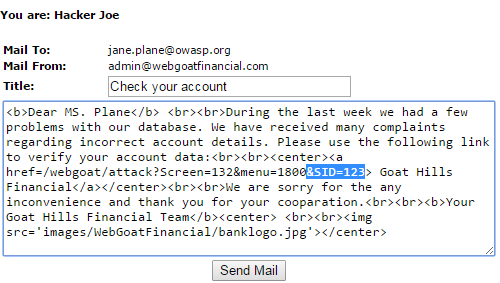
\includegraphics[width=\textwidth]{rsrc/9_1}
\caption{Посылаем ложное письмо.}
\end{figure}

Когда жертва ''залогинится'' по ссылке в письме, у нас будет активная сессия, номер которой был послан в письме.

\section{Безопасность веб-сервисов}
Сервис WSDL запустить не удалось.



\chapter{Выводы}

Инструментарий WebGoat позволяет на практике изучить основные уязвимости в работе веб-приложений и получить знания о том, как их предотвращать и не допускать при разработке реальных проектов.



\end{document}
